
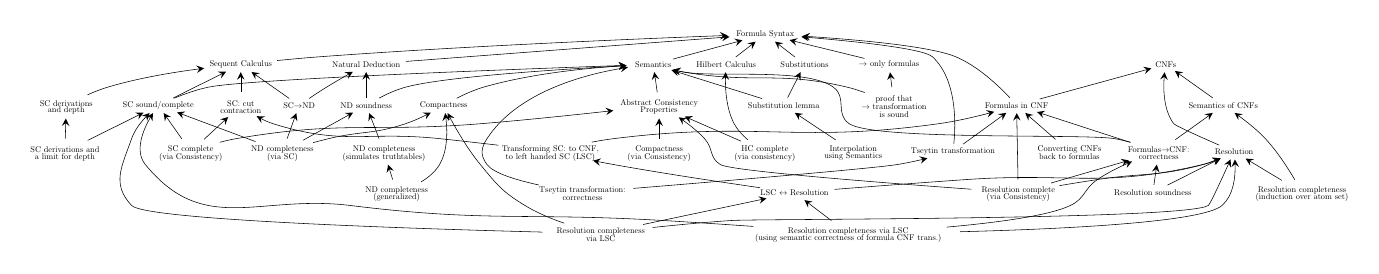
\begin{tikzpicture}[>=latex,line join=bevel,scale=0.15, every node/.style={scale=0.3}]
  \pgfsetlinewidth{1bp}
%%
\pgfsetcolor{black}
  % Edge: Compactness -> Sema
  \draw [->,-stealth,very thin] (1048.3bp,355.57bp) .. controls (1066.7bp,364.9bp) and (1090.7bp,375.86bp)  .. (1113.2bp,382.36bp) .. controls (1226.3bp,414.96bp) and (1362.8bp,428.13bp)  .. (1455.5bp,433.99bp);
  % Edge: ND -> Formulas
  \draw [->,-stealth,very thin] (926.55bp,443.99bp) .. controls (1109.8bp,457.9bp) and (1509.2bp,488.24bp)  .. (1703.2bp,502.98bp);
  % Edge: Resolution_Compl_Consistency -> Consistency
  \draw [->,-stealth,very thin] (2283.9bp,137.24bp) .. controls (2089.0bp,151.32bp) and (1706.3bp,180.75bp)  .. (1681.2bp,196.45bp) .. controls (1653.7bp,213.61bp) and (1665.1bp,234.82bp)  .. (1643.2bp,258.68bp) .. controls (1627.6bp,275.6bp) and (1608.0bp,291.26bp)  .. (1581.4bp,309.88bp);
  % Edge: Resolution_Compl_SC_Small -> LSC_Resolution
  \draw [->,-stealth,very thin] (1947.7bp,61.922bp) .. controls (1929.4bp,75.847bp) and (1908.1bp,92.063bp)  .. (1883.0bp,111.22bp);
  % Edge: SC_Depth_Limit -> SC_Depth
  \draw [->,-stealth,very thin] (109.03bp,258.77bp) .. controls (109.35bp,270.58bp) and (109.72bp,284.23bp)  .. (110.34bp,307.16bp);
  % Edge: Resolution_Compl_Consistency -> CNF_Formulas_Sema
  \draw [->,-stealth,very thin] (2475.1bp,152.19bp) .. controls (2519.7bp,165.15bp) and (2576.6bp,181.67bp)  .. (2627.2bp,196.45bp) .. controls (2635.2bp,198.79bp) and (2643.5bp,201.23bp)  .. (2661.6bp,206.53bp);
  % Edge: SCND -> ND
  \draw [->,-stealth,very thin] (694.38bp,355.15bp) .. controls (706.76bp,363.51bp) and (722.14bp,373.69bp)  .. (736.19bp,382.36bp) .. controls (753.65bp,393.14bp) and (773.29bp,404.5bp)  .. (799.21bp,419.13bp);
  % Edge: ND_Compl_SC -> SC_Sema
  \draw [->,-stealth,very thin] (565.53bp,251.64bp) .. controls (512.13bp,271.52bp) and (437.2bp,299.42bp)  .. (377.36bp,321.7bp);
  % Edge: Resolution_Compl_SC_Small -> Resolution
  \draw [->,-stealth,very thin] (2256.7bp,35.24bp) .. controls (2503.6bp,41.586bp) and (2838.2bp,57.647bp)  .. (2885.2bp,98.225bp) .. controls (2913.6bp,122.74bp) and (2917.6bp,168.47bp)  .. (2916.2bp,208.73bp);
  % Edge: LSC_Resolution -> Resolution
  \draw [->,-stealth,very thin] (1955.3bp,136.93bp) .. controls (2038.8bp,143.44bp) and (2163.0bp,152.93bp)  .. (2271.2bp,160.45bp) .. controls (2523.5bp,177.97bp) and (2592.8bp,139.21bp)  .. (2839.2bp,196.45bp) .. controls (2850.2bp,199.02bp) and (2861.7bp,203.04bp)  .. (2881.7bp,211.36bp);
  % Edge: MiniFormulas_Sema -> Sema
  \draw [->,-stealth,very thin] (2027.7bp,369.31bp) .. controls (2013.8bp,374.39bp) and (1999.2bp,379.06bp)  .. (1985.2bp,382.36bp) .. controls (1815.3bp,422.3bp) and (1766.3bp,389.24bp)  .. (1594.2bp,418.36bp) .. controls (1588.7bp,419.28bp) and (1583.1bp,420.4bp)  .. (1567.3bp,423.9bp);
  % Edge: CNF_Formulas -> CNF
  \draw [->,-stealth,very thin] (2447.7bp,353.76bp) .. controls (2518.8bp,373.24bp) and (2640.4bp,406.61bp)  .. (2715.6bp,427.26bp);
  % Edge: Substitution_Sema -> Sema
  \draw [->,-stealth,very thin] (1781.5bp,354.74bp) .. controls (1724.1bp,372.77bp) and (1631.7bp,401.74bp)  .. (1563.9bp,423.04bp);
  % Edge: Resolution_Compl_SC_Small -> SC_Sema
  \draw [->,-stealth,very thin] (1760.4bp,47.997bp) .. controls (1690.7bp,52.906bp) and (1613.8bp,58.061bp)  .. (1543.2bp,62.225bp) .. controls (1210.0bp,81.864bp) and (1124.4bp,57.444bp)  .. (793.19bp,98.225bp) .. controls (571.88bp,125.47bp) and (442.58bp,24.034bp)  .. (301.19bp,196.45bp) .. controls (274.23bp,229.32bp) and (296.15bp,280.41bp)  .. (319.52bp,320.13bp);
  % Edge: Tseytin -> CNF_Formulas
  \draw [->,-stealth,very thin] (2264.1bp,245.64bp) .. controls (2290.0bp,264.39bp) and (2330.6bp,293.82bp)  .. (2367.5bp,320.63bp);
  % Edge: SC_Sema -> Sema
  \draw [->,-stealth,very thin] (370.85bp,355.86bp) .. controls (394.19bp,365.48bp) and (424.83bp,376.63bp)  .. (453.19bp,382.36bp) .. controls (549.6bp,401.83bp) and (1218.8bp,426.37bp)  .. (1455.5bp,434.56bp);
  % Edge: ND_Compl_SC -> Compactness
  \draw [->,-stealth,very thin] (704.01bp,249.15bp) .. controls (716.38bp,252.51bp) and (729.11bp,255.81bp)  .. (741.19bp,258.68bp) .. controls (822.69bp,278.0bp) and (846.69bp,268.28bp)  .. (926.19bp,294.68bp) .. controls (943.42bp,300.4bp) and (961.59bp,308.66bp)  .. (986.43bp,321.25bp);
  % Edge: SCND -> SC
  \draw [->,-stealth,very thin] (646.44bp,355.18bp) .. controls (623.87bp,371.01bp) and (589.69bp,394.99bp)  .. (555.95bp,418.66bp);
  % Edge: Resolution_Compl_SC_Full -> Resolution
  \draw [->,-stealth,very thin] (1518.9bp,45.42bp) .. controls (1576.5bp,51.519bp) and (1645.7bp,58.153bp)  .. (1708.2bp,62.225bp) .. controls (1771.6bp,66.363bp) and (2798.9bp,63.505bp)  .. (2852.2bp,98.225bp) .. controls (2856.8bp,101.25bp) and (2885.0bp,162.66bp)  .. (2905.9bp,209.06bp);
  % Edge: LSC -> SC_Cut
  \draw [->,-stealth,very thin] (1148.4bp,242.85bp) .. controls (1103.9bp,248.13bp) and (1053.3bp,253.9bp)  .. (1007.2bp,258.68bp) .. controls (829.64bp,277.05bp) and (777.52bp,241.3bp)  .. (607.19bp,294.68bp) .. controls (597.06bp,297.85bp) and (586.81bp,302.49bp)  .. (568.27bp,312.57bp);
  % Edge: LSC -> CNF_Formulas
  \draw [->,-stealth,very thin] (1372.2bp,250.14bp) .. controls (1389.7bp,253.49bp) and (1407.9bp,256.53bp)  .. (1425.2bp,258.68bp) .. controls (1770.0bp,301.65bp) and (1862.0bp,246.61bp)  .. (2206.2bp,294.68bp) .. controls (2247.5bp,300.44bp) and (2293.1bp,311.12bp)  .. (2338.6bp,323.09bp);
  % Edge: SC_Depth -> SC
  \draw [->,-stealth,very thin] (162.18bp,363.74bp) .. controls (177.63bp,370.59bp) and (194.84bp,377.46bp)  .. (211.19bp,382.36bp) .. controls (283.73bp,404.09bp) and (368.32bp,418.01bp)  .. (442.22bp,427.61bp);
  % Edge: MiniFormulas -> Formulas
  \draw [->,-stealth,very thin] (2027.2bp,451.21bp) .. controls (1978.2bp,463.19bp) and (1908.6bp,480.24bp)  .. (1847.3bp,495.26bp);
  % Edge: CNF_To_Formula -> CNF_Formulas
  \draw [->,-stealth,very thin] (2485.5bp,257.01bp) .. controls (2465.2bp,274.72bp) and (2439.7bp,297.02bp)  .. (2412.9bp,320.42bp);
  % Edge: CNF_Formulas -> Formulas
  \draw [->,-stealth,very thin] (2375.9bp,356.84bp) .. controls (2350.9bp,383.56bp) and (2300.4bp,432.47bp)  .. (2246.2bp,455.13bp) .. controls (2183.6bp,481.32bp) and (2002.8bp,496.7bp)  .. (1878.1bp,504.73bp);
  % Edge: SC_Cut -> SC
  \draw [->,-stealth,very thin] (530.19bp,369.87bp) .. controls (530.19bp,382.07bp) and (530.19bp,395.97bp)  .. (530.19bp,418.25bp);
  % Edge: ND_Compl_Truthtable_Compact -> ND_Compl_Truthtable
  \draw [->,-stealth,very thin] (894.7bp,160.42bp) .. controls (892.15bp,168.75bp) and (889.36bp,177.88bp)  .. (883.72bp,196.35bp);
  % Edge: SC -> Formulas
  \draw [->,-stealth,very thin] (617.62bp,446.1bp) .. controls (649.56bp,449.29bp) and (685.98bp,452.67bp)  .. (719.19bp,455.13bp) .. controls (1075.1bp,481.46bp) and (1498.5bp,498.87bp)  .. (1698.6bp,506.32bp);
  % Edge: Sema_Craig -> Substitution_Sema
  \draw [->,-stealth,very thin] (1958.0bp,255.56bp) .. controls (1930.4bp,273.9bp) and (1894.8bp,297.61bp)  .. (1860.1bp,320.61bp);
  % Edge: ND_Compl_Truthtable_Compact -> Compactness
  \draw [->,-stealth,very thin] (962.96bp,154.85bp) .. controls (980.07bp,165.23bp) and (996.91bp,178.98bp)  .. (1007.2bp,196.45bp) .. controls (1027.7bp,231.34bp) and (1026.1bp,279.7bp)  .. (1020.8bp,319.96bp);
  % Edge: SC_Compl_Consistency -> SC_Cut
  \draw [->,-stealth,very thin] (442.35bp,257.3bp) .. controls (457.74bp,271.53bp) and (476.27bp,288.67bp)  .. (500.01bp,310.61bp);
  % Edge: Tseytin -> Formulas
  \draw [->,-stealth,very thin] (2241.5bp,245.96bp) .. controls (2246.0bp,289.56bp) and (2250.4bp,399.67bp)  .. (2190.2bp,455.13bp) .. controls (2168.1bp,475.44bp) and (1997.3bp,492.84bp)  .. (1875.5bp,503.04bp);
  % Edge: CNF_Formulas_Sema -> CNF_Formulas
  \draw [->,-stealth,very thin] (2665.0bp,249.75bp) .. controls (2602.3bp,270.15bp) and (2510.3bp,300.07bp)  .. (2441.2bp,322.56bp);
  % Edge: SC_Compl_Consistency -> SC_Sema
  \draw [->,-stealth,very thin] (388.67bp,258.18bp) .. controls (376.87bp,274.95bp) and (362.39bp,295.56bp)  .. (345.1bp,320.15bp);
  % Edge: Tseytin_Sema -> Sema
  \draw [->,-stealth,very thin] (1245.4bp,147.45bp) .. controls (1192.8bp,158.91bp) and (1136.9bp,175.52bp)  .. (1121.2bp,196.45bp) .. controls (1104.6bp,218.59bp) and (1106.1bp,235.48bp)  .. (1121.2bp,258.68bp) .. controls (1194.0bp,370.88bp) and (1355.8bp,413.0bp)  .. (1459.4bp,429.91bp);
  % Edge: Resolution -> CNF
  \draw [->,-stealth,very thin] (2878.4bp,243.11bp) .. controls (2836.6bp,261.4bp) and (2772.7bp,289.89bp)  .. (2769.2bp,294.68bp) .. controls (2744.9bp,327.65bp) and (2744.0bp,376.95bp)  .. (2747.4bp,418.1bp);
  % Edge: Resolution_Compl_Consistency -> CNF_Formulas
  \draw [->,-stealth,very thin] (2395.6bp,160.65bp) .. controls (2394.8bp,201.08bp) and (2393.5bp,270.84bp)  .. (2392.5bp,320.05bp);
  % Edge: Resolution_Compl_SC_Full -> Compactness
  \draw [->,-stealth,very thin] (1306.8bp,55.641bp) .. controls (1275.7bp,66.321bp) and (1241.2bp,80.506bp)  .. (1212.2bp,98.225bp) .. controls (1157.1bp,131.86bp) and (1146.3bp,146.72bp)  .. (1105.2bp,196.45bp) .. controls (1074.8bp,233.16bp) and (1047.2bp,281.23bp)  .. (1026.6bp,319.96bp);
  % Edge: CNF_Formulas_Sema -> CNF_Sema
  \draw [->,-stealth,very thin] (2773.1bp,256.14bp) .. controls (2798.3bp,274.21bp) and (2830.6bp,297.3bp)  .. (2863.0bp,320.46bp);
  % Edge: Resolution_Sound -> Resolution
  \draw [->,-stealth,very thin] (2754.5bp,147.13bp) .. controls (2787.8bp,163.92bp) and (2837.9bp,189.11bp)  .. (2882.0bp,211.37bp);
  % Edge: HC_Compl_Consistency -> HC
  \draw [->,-stealth,very thin] (1747.1bp,255.83bp) .. controls (1734.5bp,266.54bp) and (1722.0bp,279.78bp)  .. (1714.2bp,294.68bp) .. controls (1695.4bp,330.39bp) and (1692.8bp,377.83bp)  .. (1693.8bp,418.04bp);
  % Edge: ND_Compl_SC -> SCND
  \draw [->,-stealth,very thin] (641.44bp,258.77bp) .. controls (647.27bp,274.96bp) and (654.35bp,294.59bp)  .. (663.52bp,320.03bp);
  % Edge: Sema -> Formulas
  \draw [->,-stealth,very thin] (1567.4bp,449.5bp) .. controls (1610.9bp,461.28bp) and (1676.0bp,478.89bp)  .. (1734.2bp,494.63bp);
  % Edge: Substitution_Sema -> Substitution
  \draw [->,-stealth,very thin] (1842.6bp,356.99bp) .. controls (1850.1bp,371.67bp) and (1860.6bp,392.43bp)  .. (1873.8bp,418.35bp);
  % Edge: HC_Compl_Consistency -> Consistency
  \draw [->,-stealth,very thin] (1730.6bp,252.74bp) .. controls (1693.3bp,269.02bp) and (1644.5bp,290.32bp)  .. (1595.6bp,311.7bp);
  % Edge: Substitution -> Formulas
  \draw [->,-stealth,very thin] (1860.4bp,454.36bp) .. controls (1848.5bp,463.61bp) and (1833.7bp,475.08bp)  .. (1812.4bp,491.55bp);
  % Edge: Resolution_Compl_SC_Full -> LSC_Resolution
  \draw [->,-stealth,very thin] (1495.9bp,52.608bp) .. controls (1582.1bp,70.801bp) and (1703.7bp,96.485bp)  .. (1791.8bp,115.1bp);
  % Edge: Resolution_Compl -> CNF_Sema
  \draw [->,-stealth,very thin] (3059.8bp,160.26bp) .. controls (3043.6bp,187.74bp) and (3017.6bp,228.16bp)  .. (2989.2bp,258.68bp) .. controls (2969.6bp,279.72bp) and (2944.2bp,299.77bp)  .. (2915.3bp,320.5bp);
  % Edge: Resolution_Compl_SC_Full -> SC_Sema
  \draw [->,-stealth,very thin] (1254.9bp,34.382bp) .. controls (960.97bp,41.962bp) and (301.53bp,62.837bp)  .. (268.19bp,98.225bp) .. controls (219.29bp,150.13bp) and (244.55bp,191.4bp)  .. (268.19bp,258.68bp) .. controls (275.39bp,279.18bp) and (290.33bp,298.32bp)  .. (311.34bp,320.21bp);
  % Edge: Compactness_Consistency -> Consistency
  \draw [->,-stealth,very thin] (1534.2bp,258.77bp) .. controls (1534.2bp,270.58bp) and (1534.2bp,284.23bp)  .. (1534.2bp,307.16bp);
  % Edge: ND_Sound -> Sema
  \draw [->,-stealth,very thin] (861.84bp,355.92bp) .. controls (879.98bp,365.38bp) and (903.73bp,376.34bp)  .. (926.19bp,382.36bp) .. controls (1022.3bp,408.11bp) and (1308.7bp,425.84bp)  .. (1456.0bp,433.63bp);
  % Edge: LSC_Resolution -> LSC
  \draw [->,-stealth,very thin] (1776.6bp,140.89bp) .. controls (1689.1bp,153.42bp) and (1547.1bp,174.56bp)  .. (1425.2bp,196.45bp) .. controls (1412.4bp,198.75bp) and (1399.0bp,201.28bp)  .. (1375.7bp,205.88bp);
  % Edge: Resolution_Compl -> Resolution
  \draw [->,-stealth,very thin] (3028.7bp,158.54bp) .. controls (3003.7bp,173.62bp) and (2973.7bp,191.71bp)  .. (2941.9bp,210.87bp);
  % Edge: SC_Sema -> SC
  \draw [->,-stealth,very thin] (367.59bp,356.08bp) .. controls (400.67bp,372.49bp) and (450.19bp,397.05bp)  .. (495.1bp,419.33bp);
  % Edge: ND_Compl_Truthtable -> ND_Sound
  \draw [->,-stealth,very thin] (862.1bp,258.77bp) .. controls (855.82bp,274.96bp) and (848.21bp,294.59bp)  .. (838.35bp,320.03bp);
  % Edge: Consistency -> Sema
  \draw [->,-stealth,very thin] (1529.7bp,369.87bp) .. controls (1528.0bp,382.2bp) and (1526.0bp,396.26bp)  .. (1522.8bp,418.25bp);
  % Edge: Resolution_Sound -> CNF_Formulas_Sema
  \draw [->,-stealth,very thin] (2721.8bp,147.81bp) .. controls (2723.4bp,158.71bp) and (2725.4bp,172.95bp)  .. (2728.7bp,196.42bp);
  % Edge: ND_Sound -> ND
  \draw [->,-stealth,very thin] (831.19bp,356.99bp) .. controls (831.19bp,371.4bp) and (831.19bp,391.66bp)  .. (831.19bp,418.35bp);
  % Edge: Resolution_Compl_SC_Small -> CNF_Formulas_Sema
  \draw [->,-stealth,very thin] (2224.5bp,46.318bp) .. controls (2341.5bp,56.742bp) and (2468.8bp,73.289bp)  .. (2521.2bp,98.225bp) .. controls (2557.3bp,115.42bp) and (2553.1bp,138.0bp)  .. (2586.2bp,160.45bp) .. controls (2608.9bp,175.88bp) and (2635.8bp,189.33bp)  .. (2669.6bp,204.03bp);
  % Edge: CNF_Sema -> CNF
  \draw [->,-stealth,very thin] (2862.9bp,356.53bp) .. controls (2839.6bp,373.08bp) and (2805.1bp,397.63bp)  .. (2772.2bp,421.11bp);
  % Edge: HC -> Formulas
  \draw [->,-stealth,very thin] (1718.4bp,454.73bp) .. controls (1730.3bp,463.91bp) and (1744.9bp,475.22bp)  .. (1765.9bp,491.48bp);
  % Edge: Resolution_Compl_Consistency -> Resolution
  \draw [->,-stealth,very thin] (2494.7bp,145.88bp) .. controls (2524.1bp,150.7bp) and (2556.5bp,155.9bp)  .. (2586.2bp,160.45bp) .. controls (2698.5bp,177.63bp) and (2729.6bp,166.45bp)  .. (2839.2bp,196.45bp) .. controls (2849.9bp,199.39bp) and (2861.1bp,203.47bp)  .. (2880.8bp,211.62bp);
  % Edge: MiniFormulas_Sema -> MiniFormulas
  \draw [->,-stealth,very thin] (2092.8bp,382.46bp) .. controls (2091.8bp,391.03bp) and (2090.7bp,399.81bp)  .. (2088.5bp,417.94bp);
  % Edge: Tseytin_Sema -> Tseytin
  \draw [->,-stealth,very thin] (1472.3bp,139.25bp) .. controls (1670.1bp,155.45bp) and (2044.5bp,186.75bp)  .. (2105.2bp,196.45bp) .. controls (2125.9bp,199.75bp) and (2148.1bp,204.44bp)  .. (2178.2bp,211.5bp);
  % Edge: SC_Compl_Consistency -> Consistency
  \draw [->,-stealth,very thin] (480.03bp,249.92bp) .. controls (492.94bp,253.36bp) and (506.39bp,256.48bp)  .. (519.19bp,258.68bp) .. controls (777.69bp,302.93bp) and (846.8bp,273.25bp)  .. (1108.2bp,294.68bp) .. controls (1211.7bp,303.16bp) and (1329.1bp,315.45bp)  .. (1424.4bp,325.96bp);
  % Edge: CNF_Formulas_Sema -> Sema
  \draw [->,-stealth,very thin] (2665.6bp,249.9bp) .. controls (2652.9bp,253.36bp) and (2639.8bp,256.51bp)  .. (2627.2bp,258.68bp) .. controls (2557.3bp,270.74bp) and (2048.3bp,254.11bp)  .. (1990.2bp,294.68bp) .. controls (1955.4bp,318.98bp) and (1986.5bp,357.3bp)  .. (1952.2bp,382.36bp) .. controls (1887.6bp,429.53bp) and (1673.0bp,404.68bp)  .. (1594.2bp,418.36bp) .. controls (1588.7bp,419.31bp) and (1583.1bp,420.44bp)  .. (1567.3bp,423.96bp);
  % Edge: SC_Depth_Limit -> SC_Sema
  \draw [->,-stealth,very thin] (162.7bp,254.56bp) .. controls (200.98bp,273.52bp) and (251.55bp,298.57bp)  .. (296.72bp,320.95bp);
  % Edge: ND_Compl_SC -> ND_Sound
  \draw [->,-stealth,very thin] (679.61bp,254.85bp) .. controls (713.79bp,273.71bp) and (758.69bp,298.5bp)  .. (799.82bp,321.2bp);
  % Node: Resolution_Compl_Consistency
\begin{scope}
  \definecolor{strokecol}{rgb}{0.0,0.0,0.0};
  \pgfsetstrokecolor{strokecol}
  \draw (2396.19bp,134.54bp) node {Resolution complete};
  \draw (2396.19bp,116.54bp) node {(via Consistency)};
\end{scope}
  % Node: ND_Compl_SC
\begin{scope}
  \definecolor{strokecol}{rgb}{0.0,0.0,0.0};
  \pgfsetstrokecolor{strokecol}
  \draw (630.19bp,232.76bp) node {ND completeness};
  \draw (630.19bp,214.76bp) node {(via SC)};
\end{scope}
  % Node: CNF_Formulas
\begin{scope}
  \definecolor{strokecol}{rgb}{0.0,0.0,0.0};
  \pgfsetstrokecolor{strokecol}
  \draw (2392.2bp,338.52bp) node {Formulas in CNF};
\end{scope}
  % Node: Substitution_Sema
\begin{scope}
  \definecolor{strokecol}{rgb}{0.0,0.0,0.0};
  \pgfsetstrokecolor{strokecol}
  \draw (1833.2bp,338.52bp) node {Substitution lemma};
\end{scope}
  % Node: CNF_Formulas_Sema
\begin{scope}
  \definecolor{strokecol}{rgb}{0.0,0.0,0.0};
  \pgfsetstrokecolor{strokecol}
  \draw (2733.19bp,232.76bp) node {Formulas$\rightarrow$CNF:};
  \draw (2733.19bp,214.76bp) node {correctness};
\end{scope}
  % Node: LSC_Resolution
\begin{scope}
  \definecolor{strokecol}{rgb}{0.0,0.0,0.0};
  \pgfsetstrokecolor{strokecol}
  \draw (1859.2bp,129.34bp) node {LSC $\leftrightarrow$ Resolution};
\end{scope}
  % Node: HC
\begin{scope}
  \definecolor{strokecol}{rgb}{0.0,0.0,0.0};
  \pgfsetstrokecolor{strokecol}
  \draw (1695.2bp,436.74bp) node {Hilbert Calculus};
\end{scope}
  % Node: SCND
\begin{scope}
  \definecolor{strokecol}{rgb}{0.0,0.0,0.0};
  \pgfsetstrokecolor{strokecol}
  \draw (670.19bp,338.52bp) node {SC$\rightarrow$ND};
\end{scope}
  % Node: Formulas
\begin{scope}
  \definecolor{strokecol}{rgb}{0.0,0.0,0.0};
  \pgfsetstrokecolor{strokecol}
  \draw (1789.2bp,509.51bp) node {Formula Syntax};
\end{scope}
  % Node: SC_Compl_Consistency
\begin{scope}
  \definecolor{strokecol}{rgb}{0.0,0.0,0.0};
  \pgfsetstrokecolor{strokecol}
  \draw (410.19bp,232.76bp) node {SC complete};
  \draw (410.19bp,214.76bp) node {(via Consistency)};
\end{scope}
  % Node: ND
\begin{scope}
  \definecolor{strokecol}{rgb}{0.0,0.0,0.0};
  \pgfsetstrokecolor{strokecol}
  \draw (831.19bp,436.74bp) node {Natural Deduction};
\end{scope}
  % Node: Tseytin
\begin{scope}
  \definecolor{strokecol}{rgb}{0.0,0.0,0.0};
  \pgfsetstrokecolor{strokecol}
  \draw (2239.2bp,227.56bp) node {Tseytin transformation};
\end{scope}
  % Node: MiniFormulas
\begin{scope}
  \definecolor{strokecol}{rgb}{0.0,0.0,0.0};
  \pgfsetstrokecolor{strokecol}
  \draw (2086.2bp,436.74bp) node {$\rightarrow$ only formulas};
\end{scope}
  % Node: ND_Compl_Truthtable_Compact
\begin{scope}
  \definecolor{strokecol}{rgb}{0.0,0.0,0.0};
  \pgfsetstrokecolor{strokecol}
  \draw (904.19bp,134.54bp) node {ND completeness};
  \draw (904.19bp,116.54bp) node {(generalized)};
\end{scope}
  % Node: Substitution
\begin{scope}
  \definecolor{strokecol}{rgb}{0.0,0.0,0.0};
  \pgfsetstrokecolor{strokecol}
  \draw (1883.2bp,436.74bp) node {Substitutions};
\end{scope}
  % Node: ND_Sound
\begin{scope}
  \definecolor{strokecol}{rgb}{0.0,0.0,0.0};
  \pgfsetstrokecolor{strokecol}
  \draw (831.19bp,338.52bp) node {ND soundness};
\end{scope}
  % Node: Resolution_Compl_SC_Small
\begin{scope}
  \definecolor{strokecol}{rgb}{0.0,0.0,0.0};
  \pgfsetstrokecolor{strokecol}
  \draw (1988.19bp,36.31bp) node {Resolution completeness via LSC};
  \draw (1988.19bp,18.31bp) node {(using semantic correctness of formula CNF trans.)};
\end{scope}
  % Node: CNF_To_Formula
\begin{scope}
  \definecolor{strokecol}{rgb}{0.0,0.0,0.0};
  \pgfsetstrokecolor{strokecol}
  \draw (2519.19bp,232.76bp) node {Converting CNFs};
  \draw (2519.19bp,214.76bp) node {back to formulas};
\end{scope}
  % Node: Sema_Craig
\begin{scope}
  \definecolor{strokecol}{rgb}{0.0,0.0,0.0};
  \pgfsetstrokecolor{strokecol}
  \draw (2000.19bp,232.76bp) node {Interpolation};
  \draw (2000.19bp,214.76bp) node {using Semantics};
\end{scope}
  % Node: MiniFormulas_Sema
\begin{scope}
  \definecolor{strokecol}{rgb}{0.0,0.0,0.0};
  \pgfsetstrokecolor{strokecol}
  \draw (2098.19bp,352.72bp) node {proof that};
  \draw (2098.19bp,334.72bp) node {$\rightarrow$ transformation};
  \draw (2098.19bp,316.72bp) node {is sound};
\end{scope}
  % Node: ND_Compl_Truthtable
\begin{scope}
  \definecolor{strokecol}{rgb}{0.0,0.0,0.0};
  \pgfsetstrokecolor{strokecol}
  \draw (874.19bp,232.76bp) node {ND completeness};
  \draw (874.19bp,214.76bp) node {(simulates truthtables)};
\end{scope}
  % Node: Sema
\begin{scope}
  \definecolor{strokecol}{rgb}{0.0,0.0,0.0};
  \pgfsetstrokecolor{strokecol}
  \draw (1520.2bp,436.74bp) node {Semantics};
\end{scope}
  % Node: CNF
\begin{scope}
  \definecolor{strokecol}{rgb}{0.0,0.0,0.0};
  \pgfsetstrokecolor{strokecol}
  \draw (2750.2bp,436.74bp) node {CNFs};
\end{scope}
  % Node: SC
\begin{scope}
  \definecolor{strokecol}{rgb}{0.0,0.0,0.0};
  \pgfsetstrokecolor{strokecol}
  \draw (530.19bp,436.74bp) node {Sequent Calculus};
\end{scope}
  % Node: CNF_Sema
\begin{scope}
  \definecolor{strokecol}{rgb}{0.0,0.0,0.0};
  \pgfsetstrokecolor{strokecol}
  \draw (2888.2bp,338.52bp) node {Semantics of CNFs};
\end{scope}
  % Node: Compactness
\begin{scope}
  \definecolor{strokecol}{rgb}{0.0,0.0,0.0};
  \pgfsetstrokecolor{strokecol}
  \draw (1017.2bp,338.52bp) node {Compactness};
\end{scope}
  % Node: SC_Depth_Limit
\begin{scope}
  \definecolor{strokecol}{rgb}{0.0,0.0,0.0};
  \pgfsetstrokecolor{strokecol}
  \draw (108.19bp,232.76bp) node {SC derivations and};
  \draw (108.19bp,214.76bp) node {a limit for depth};
\end{scope}
  % Node: Consistency
\begin{scope}
  \definecolor{strokecol}{rgb}{0.0,0.0,0.0};
  \pgfsetstrokecolor{strokecol}
  \draw (1534.19bp,343.72bp) node {Abstract Consistency};
  \draw (1534.19bp,325.72bp) node {Properties};
\end{scope}
  % Node: Resolution_Compl
\begin{scope}
  \definecolor{strokecol}{rgb}{0.0,0.0,0.0};
  \pgfsetstrokecolor{strokecol}
  \draw (3077.19bp,134.54bp) node {Resolution completeness};
  \draw (3077.19bp,116.54bp) node {(induction over atom set)};
\end{scope}
  % Node: Resolution_Sound
\begin{scope}
  \definecolor{strokecol}{rgb}{0.0,0.0,0.0};
  \pgfsetstrokecolor{strokecol}
  \draw (2719.2bp,129.34bp) node {Resolution soundness};
\end{scope}
  % Node: Resolution
\begin{scope}
  \definecolor{strokecol}{rgb}{0.0,0.0,0.0};
  \pgfsetstrokecolor{strokecol}
  \draw (2914.2bp,227.56bp) node {Resolution};
\end{scope}
  % Node: LSC
\begin{scope}
  \definecolor{strokecol}{rgb}{0.0,0.0,0.0};
  \pgfsetstrokecolor{strokecol}
  \draw (1273.19bp,232.76bp) node {Transforming SC: to CNF,};
  \draw (1273.19bp,214.76bp) node {to left handed SC (LSC)};
\end{scope}
  % Node: SC_Sema
\begin{scope}
  \definecolor{strokecol}{rgb}{0.0,0.0,0.0};
  \pgfsetstrokecolor{strokecol}
  \draw (332.19bp,338.52bp) node {SC sound/complete};
\end{scope}
  % Node: Resolution_Compl_SC_Full
\begin{scope}
  \definecolor{strokecol}{rgb}{0.0,0.0,0.0};
  \pgfsetstrokecolor{strokecol}
  \draw (1394.19bp,36.31bp) node {Resolution completeness};
  \draw (1394.19bp,18.31bp) node {via LSC};
\end{scope}
  % Node: SC_Depth
\begin{scope}
  \definecolor{strokecol}{rgb}{0.0,0.0,0.0};
  \pgfsetstrokecolor{strokecol}
  \draw (111.19bp,343.72bp) node {SC derivations};
  \draw (111.19bp,325.72bp) node {and depth};
\end{scope}
  % Node: HC_Compl_Consistency
\begin{scope}
  \definecolor{strokecol}{rgb}{0.0,0.0,0.0};
  \pgfsetstrokecolor{strokecol}
  \draw (1788.19bp,232.76bp) node {HC complete};
  \draw (1788.19bp,214.76bp) node {(via consistency)};
\end{scope}
  % Node: Compactness_Consistency
\begin{scope}
  \definecolor{strokecol}{rgb}{0.0,0.0,0.0};
  \pgfsetstrokecolor{strokecol}
  \draw (1534.19bp,232.76bp) node {Compactness};
  \draw (1534.19bp,214.76bp) node {(via Consistency)};
\end{scope}
  % Node: Tseytin_Sema
\begin{scope}
  \definecolor{strokecol}{rgb}{0.0,0.0,0.0};
  \pgfsetstrokecolor{strokecol}
  \draw (1350.19bp,134.54bp) node {Tseytin transformation:};
  \draw (1350.19bp,116.54bp) node {correctness};
\end{scope}
  % Node: SC_Cut
\begin{scope}
  \definecolor{strokecol}{rgb}{0.0,0.0,0.0};
  \pgfsetstrokecolor{strokecol}
  \draw (530.19bp,343.72bp) node {SC: cut};
  \draw (530.19bp,325.72bp) node {contraction};
\end{scope}
%
\end{tikzpicture}

